\documentclass{beamer}
\usepackage{minted}
% \usepackage{beamerthemesplit} // Activate for custom appearance
\definecolor{links}{HTML}{2A1B81}
\hypersetup{urlcolor=links}
\hypersetup{colorlinks,urlcolor=links}
\title{Performing Analysis with IPython}
\author{Piti Ongmongkolkul \& Chih-hsiang Cheng}
\date{\today}
\definecolor{bg}{rgb}{0.5,0.5,0.5}
\begin{document}

\frame{\titlepage}

\section[Outline]{}

\frame{
\frametitle{Outline}
\begin{itemize}
	\item What do we in an analysis.
	\item ROOT and what's missing.
	\item Python
	\item IPython Notebook
	\item Reading RootFile
\end{itemize}
}

\frame{
	\frametitle{What do we do in an analysis?}
	\begin{itemize}
	\item We read a ROOT file.(At least that's what framework gets us)
	\item We plot stuff.
	\item We perform multivariate technique. (Cuts, classifiers etc.)
	\item We use MINUIT or ROOFIT or your favorite fitting package. To extract observables.
	\end{itemize}
}

\frame{
	\frametitle{ROOT}
	\begin{itemize}
	\item De facto high-energy physics analysis environment. Has been around forever.
	\item IO (writing reading file). This is done right. I'd say it's the best you can find commercial or free.
	\item You can Plot stuff.
	\item Has TMVA. SPR supports ROOT out of the box(ish).
	\item Written in C++. Fast...(somewhat). You can write C++ and link against it.
	\item Has interactive environment. The notorious CINT. This will be change Cling soon. But, it will still be a C++ interpreter. TBrowser doesn't help much.
	\end{itemize}
}

\begin{frame}[fragile]{The Language}
	\begin{itemize}
	\item A lot of problem with ROOT is not really ROOT problem.
	\item C++ is a very verbose static type language. Good for other things but not a dynamic work like data analysis.
	\item C++. Repeat yourself like crazy.
		\begin{itemize}
		\item
		\begin{minted}[bgcolor=bg, frame=lines]{cpp}
			TFile f("myfile.root");
			TTree* tree = dynamic_cast<TTree*>f.Get("tree");
			float x;
			tree->SetBranchAddress("x",&x);
			tree->GetEntry(10);
			cout << x << endl;
		\end{minted}
		\end{itemize}
	\item Python. root\_numpy. \url{https://github.com/rootpy/root_numpy}
		\begin{itemize}
			\item 
			\begin{minted}[bgcolor=bg, frame=lines]{python}
				data = root2rec("myfile.root")#treename is optional
				print data.x[10]
			\end{minted}
			\item There is PyROOT. But it is very slow for doing basic stuff like reading file. We wrote a library to do this as fast as C++. There is also rootpy which use root\_numpy as backend.
		\end{itemize}
	\end{itemize}
\end{frame}

\begin{frame}[fragile]{Interactive Environment}
	\fontsize{10}{10}\selectfont
	\begin{columns}
	\begin{column}{0.5\textwidth}
		\begin{itemize}
		\item ROOT interactive environment is not so good for doing analysis. This applied to both new TBrowser and command prompt environment.
		\item IPython Notebook environment. 
		\item \url{http://ipython.org/}
		\item Mathematica. Maple. Matlab. Sage.
		\item Type command. See output. Edit command. See output.
		\item Immediate inline feedback is the key. No separate windows.
		\item Save it along with output. Come back and view/re-execute later.

		\end{itemize}
	\end{column}
	\begin{column}{0.5\textwidth}
		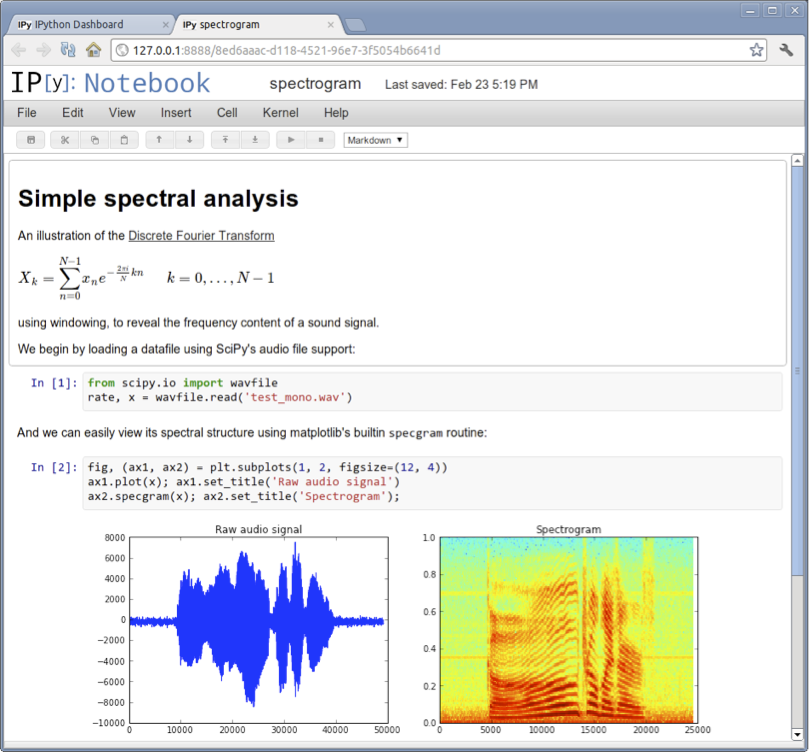
\includegraphics[width=\textwidth]{pic/ipy-notebook-spectral.png}
	\end{column}
	\end{columns}
\end{frame}

\begin{frame}{Ugly Plot}
	\begin{columns}
	\begin{column}{0.6\textwidth}
	\begin{itemize}	
	\item Needs tons of work to make
	it looks OK. They changed it recently though.
	\item Gray background by default. How many of you have Gray
			background in your slides?
	\item Default color for COLZ.
		\begin{itemize}
			\item Legend says they are the 16 color supported 
			by color screen back then.
		\end{itemize}
	\item No transparent color!!

	\item Matplotlib. Python plotting library.
		\url{http://matplotlib.org/}
	\item huge Gallery 
	
	\url{http://matplotlib.org/gallery.html}

	\end{itemize}
	\end{column}
	\begin{column}{0.4\textwidth}
		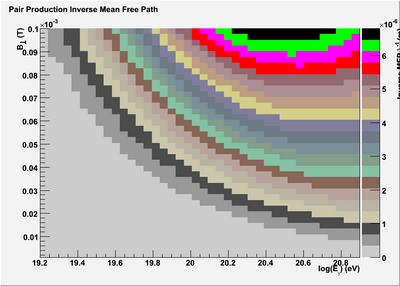
\includegraphics[width=\textwidth]{pic/default_palette_400.png}
		
		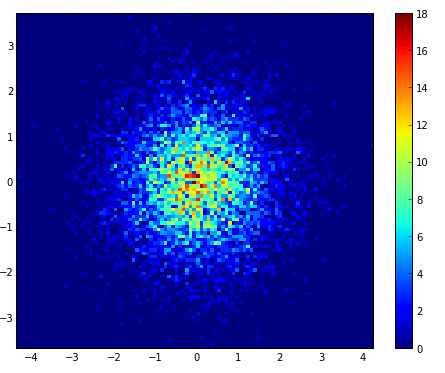
\includegraphics[width=\textwidth]{pic/hist2d-matplotlib.png}

	\end{column}
	\end{columns}
\end{frame}

\begin{frame}[fragile]{Horrible Plotting Syntax}
	\begin{itemize}
	\item ROOT. Black magic.
	\begin{minted}[fontsize=\footnotesize, frame=lines]{c++}
		tree->Draw("x");
		TH1F *xhist = (TH1F*)gPad->GetPrimitive("htemp");
		htemp->SetLineColor(kRed);
		tree->Draw("y>>anotherhist","same");
		TH1F *yhist = (TH1F*)gPad->GetPrimitive("anotherhist");
		yhist->SetLineColor(kBlue);
		htemp->SetTitle("Magic!!!");
		Legend* leg = new TLegend(0.1,0.7,0.48,0.9);
		leg->SetHeader("The Legend Title");
		leg->AddEntry(xhist,"x");
		leg->AddEntry(yhist,"y");
		leg->Draw();
	\end{minted}
	\item Matplotlib. Much more intuitive.
		\begin{minted}[fontsize=\footnotesize, frame=lines]{python}
		hist(tree.x, label="x", color="red", hist_type="step")
		hist(tree.y, label="y", color="blue", hist_type="step")
		title("That is the way it should be")
		legend(loc="upper right") #yep that simple.
		\end{minted}
	\end{itemize}
\end{frame}

\begin{frame}[fragile]{Multivariate Analysis and Fitting}
	\begin{itemize}
	\item Python has tons of packages to do multivariate analysis.
		\begin{itemize}
			\item Most popular one is scikit-learn
				\url{http://scikit-learn.org/}
			\item A Bunch of neural network library too.
		\end{itemize}
	\item Fitting takes advantage of python introspection. It
	automatically recognize function argument name. No need to repeat
	yourself.
	\begin{minted}[frame=lines]{python}
		def f(x,y,z):
		    return (x-2)**2+(y-3)**2+(z-4)**2
		m = Minuit(f)
		m.migrad()
		print m.values #{"x":2.,"y":3.,"z":4.}
	\end{minted}
		\begin{itemize}
			\item \url{https://github.com/piti118/RTMinuit}
			\item \url{https://github.com/piti118/dist_fit}
				\begin{minted}[frame=lines]{python}
					lh = BinLH(pdf,data)#automatically read pdf arguments
					m = Minuit(lh)
					m.migrad()
				\end{minted}
		\end{itemize}
	\end{itemize}
\end{frame}


\begin{frame}[fragile]{Tutorial}
	Let's see how we can use all these to create a better workflow.
\end{frame}

\end{document}
